\documentclass[10pt,twocolumn,letterpaper]{article}

\usepackage{aicourse}
\usepackage{times}
\usepackage{epsfig}
\usepackage{graphicx}
\usepackage{amsmath}
\usepackage{amssymb}
\usepackage{tikz}
\usetikzlibrary{arrows.meta,positioning}

\usepackage[breaklinks=true,bookmarks=false]{hyperref}

\aicoursefinalcopy

\setcounter{page}{1}


\begin{document}

%%%%%%%%% TITLE
\title{A Three-Layer Framework for Fake News Detection, Verification, and Explanation}

\author{Kayleb Elorm Aston Parkes\\
{\tt\small ec251170@qmul.ac.uk}
\and
Eric Kamalendran\\
{\tt\small ec251192@qmul.ac.uk}
\and
William Finlay McKie\\
{\tt\small ec251168@qmul.ac.uk}
}

\maketitle

%%%%%%%%% ABSTRACT
\begin{abstract}
The proliferation of misinformation on online platforms creates a need for
automated systems that are accurate without concealing uncertainty or conflicting
evidence. We present a three-layer framework that combines a RoBERTa classifier
fine-tuned with Low-Rank Adaptation, Monte Carlo (MC) Dropout uncertainty
estimation, live web retrieval with DeBERTa natural-language inference (NLI), and
a structured explanation agent. The deployed pipeline has no confidence gate:
classification and verification run for every input, the classifier label remains
final, and verification is displayed as supporting context. Selective escalation
is evaluated separately as an offline experiment. On the held-out WELFake test
split, RoBERTa-LoRA reached 0.9957 accuracy and macro-$F_1$; 30-pass MC Dropout
reached 0.9967 accuracy but did not improve expected calibration error. Deferring
the 100 highest-entropy articles retained 98.94\% coverage at 99.88\% accuracy.
Conversely, direct NLI override reduced accuracy from 76.0\% to 64.0\% in the
100-article low-confidence bucket. The public Gradio deployment demonstrates the
complete classifier, verification, and explanation path. These findings support
uncertainty for routing and evidence for review, but not unthresholded automatic
reclassification.
\end{abstract}

%%%%%%%%% BODY TEXT
\section{Introduction}
Digital media has made news easier to distribute while also increasing the speed
and scale of misinformation. False stories can influence elections, public health,
and trust in institutions, and false news has been observed to diffuse farther and
faster than truthful news online \cite{vosoughi2018spread}. Because manual review
cannot cover the volume of newly published material, automated detection can serve
as a scalable aid to human fact-checkers.

Transformer encoders such as RoBERTa provide strong contextual text
representations, but a single high-confidence prediction can still be wrong or
poorly calibrated. Content-only classification also cannot establish whether an
article agrees with current external evidence. A useful system should therefore
separate the classifier's judgement, its uncertainty, and the evidence retrieved
for review rather than presenting one opaque binary answer.

We implement a three-layer framework. First, RoBERTa-LoRA classifies a full news
article as real or fake and MC Dropout estimates predictive uncertainty. Second,
live DuckDuckGo (DDG) retrieval supplies snippets to a FEVER-tuned DeBERTa NLI
model. Third, an Anthropic explanation agent verbalises only the structured
classifier, uncertainty, and verification signals. The deployed design has
\emph{no confidence gate}: classification and verification run unconditionally and
in parallel for every input, and the classifier label is always final. The NLI
verdict is supporting context, not an override. Selective deferral and direct NLI
override are examined only as offline experiments on held-out WELFake articles.
LIAR was inspected during dataset selection but was never used for training or
evaluation. The contribution is therefore an in-dataset WELFake study of
classification, calibration, uncertainty-guided retention, evidence reliability,
and explanation faithfulness, together with a public end-to-end deployment.

\section{Related Work}
Early fake-news detectors commonly used support-vector machines, Naive Bayes,
logistic regression, and random forests with handcrafted lexical or syntactic
features \cite{shu2017fake}. These methods can expose useful word-frequency
signals, but manual features often transfer poorly across domains and cannot
represent long-range context.

The Transformer replaced recurrence with self-attention for modelling long-range
dependencies \cite{vaswani2017attention}. BERT introduced bidirectional
pretraining \cite{devlin2019bert}, while RoBERTa removed the next-sentence
prediction objective, expanded pretraining data, and improved the training
procedure \cite{liu2019roberta}. RoBERTa is therefore used here as a stronger
contextual encoder. Low-Rank Adaptation (LoRA) reduces the cost of fine-tuning by
learning small low-rank updates while freezing the pretrained weights
\cite{hu2022lora}.

Modern neural networks can nevertheless be poorly calibrated
\cite{guo2017calibration}. MC Dropout keeps dropout active for repeated stochastic
forward passes and provides a practical approximation to Bayesian model averaging
\cite{gal2016dropout}. Its pass-to-pass variation supports predictive-entropy and
mutual-information estimates, while selective-classification research motivates
deferring uncertain cases instead of forcing every automated prediction
\cite{geifman2017selective}.

External verification addresses a different limitation: textual style alone does
not determine factual truth. FEVER formalised retrieval followed by entailment for
claim verification \cite{thorne-etal-2018-fever}, and later systems combined
retrieval with BERT-based evidence aggregation
\cite{hanselowski-etal-2018-ukp,soleimani-etal-2020-bert}. Natural-language
inference benchmarks such as SNLI support semantic reasoning over
premise--hypothesis pairs \cite{bowman2015snli}; DeBERTa strengthens this reasoning
through disentangled attention and enhanced positional encoding
\cite{he2021deberta}.

Dataset choice also bounds what can be claimed. LIAR contains short political
statements with six truthfulness labels \cite{wang2017liar}, whereas WELFake
contains full news articles with binary labels \cite{verma2021welfake}. The latter
matches this project's article-level input and is the sole source used for training
and reported evaluation. Near-ceiling in-dataset scores may still reflect shortcut
features rather than transferable veracity cues \cite{geirhos2020shortcut}. Our
work connects contextual classification, uncertainty estimation, live evidence,
and structured explanation while evaluating where those signals agree and fail.

\section{Proposed Method}
\subsection{System Overview}
Figure~\ref{fig:pipeline} summarises the deployed no-gate architecture. Each article
is sent in parallel to the classifier and retrieval--NLI branches. The deterministic
label remains final; MC Dropout supplies a stability signal, while the NLI verdict
enters the explanation agent as supporting context only.

\begin{figure*}[t]
  \centering
  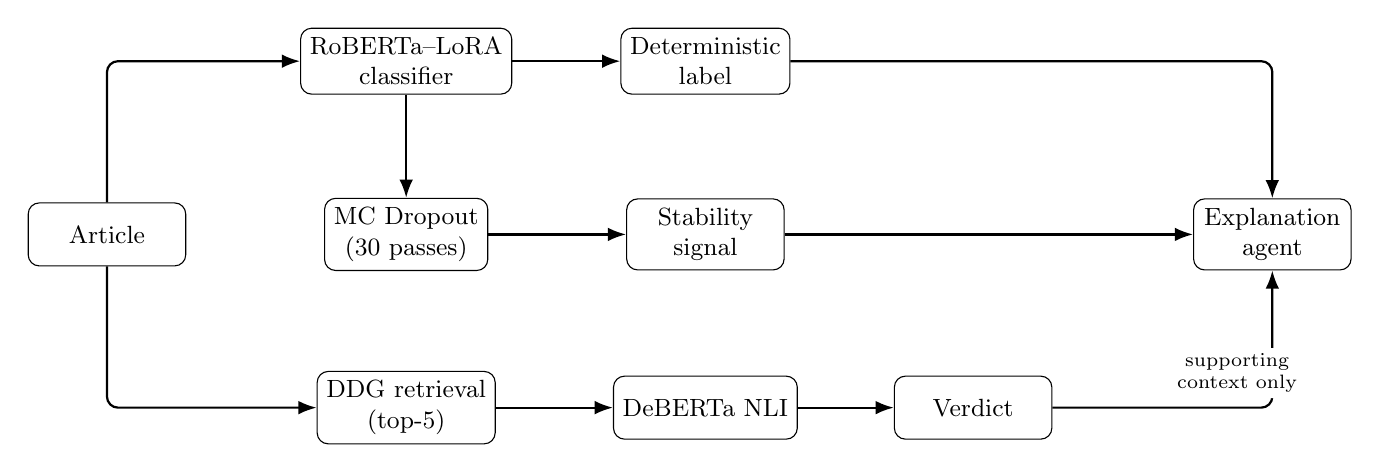
\begin{tikzpicture}[
    node distance=8mm and 12mm,
    block/.style={draw, rounded corners, align=center, minimum height=8mm,
                  minimum width=20mm, font=\small},
    signal/.style={draw, rounded corners, align=center, minimum height=8mm,
                   minimum width=20mm, font=\small},
    flow/.style={draw, -{Latex}, thick, rounded corners=4pt}
  ]
    \node[block] (article) at (0,0) {Article};
    \node[block] (classifier) at (3.8,2.2) {RoBERTa--LoRA\\classifier};
    \node[signal] (label) at (7.6,2.2) {Deterministic\\label};
    \node[block] (mc) at (3.8,0) {MC Dropout\\(30 passes)};
    \node[signal] (stability) at (7.6,0) {Stability\\signal};
    \node[block] (retrieval) at (3.8,-2.2) {DDG retrieval\\(top-$5$)};
    \node[block] (nli) at (7.6,-2.2) {DeBERTa NLI};
    \node[signal] (verdict) at (11.0,-2.2) {Verdict};
    \node[block] (explanation) at (14.8,0) {Explanation\\agent};

    \draw[flow] (article.north) |- (classifier.west);
    \draw[flow] (article.south) |- (retrieval.west);
    \draw[flow] (classifier.east) -- (label.west);
    \draw[flow] (classifier.south) -- (mc.north);
    \draw[flow] (mc.east) -- (stability.west);
    \draw[flow] (retrieval.east) -- (nli.west);
    \draw[flow] (nli.east) -- (verdict.west);
    \draw[flow] (label.east) -| (explanation.north);
    \draw[flow] (stability.east) -- (explanation.west);
    \draw[flow] (verdict.east) -|
      node[pos=0.42, above=3pt, align=center, fill=white, inner sep=2pt,
           font=\scriptsize] {supporting\\context only}
      (explanation.south);
  \end{tikzpicture}
  \caption{Deployed three-layer pipeline. Classification and verification run in
  parallel for every article. MC Dropout supplies stability beside the fixed
  deterministic label; the NLI verdict is advisory context for explanation and
  never overrides that label.}
  \label{fig:pipeline}
\end{figure*}

\subsection{Problem Formulation}
Fake-news detection is treated as binary document classification. Given
\begin{equation}
  \mathcal{D}=\{(x_i,y_i)\}_{i=1}^{N}, \qquad y_i\in\{0,1\},
\end{equation}
where 0 denotes real and 1 denotes fake, each document $x_i$ concatenates an
article title and body. The objective is to estimate $p(y\mid x)$ for unseen
articles rather than memorising surface patterns in the training set.

\subsection{RoBERTa with Low-Rank Adaptation}
A pretrained RoBERTa encoder $f_{\theta}$ maps a tokenised document to a pooled
representation, and a classification head $g_{\phi}$ maps that representation to
$C=2$ logits:
\begin{align}
  h &= f_{\theta}(x)\in\mathbb{R}^{d}, &
  z &= g_{\phi}(h)\in\mathbb{R}^{C}, \\
  p(y=c\mid x) &= \frac{\exp(z_c)}{\sum_{j=1}^{C}\exp(z_j)}.
\end{align}
Training minimises cross-entropy,
\begin{equation}
  \mathcal{L}_{\mathrm{CE}}=-\frac{1}{N}\sum_{i=1}^{N}\sum_{c=1}^{C}
  \mathbf{1}[y_i=c]\log p(y=c\mid x_i).
\end{equation}
A contextual encoder is preferred to logistic regression because it represents
word order and meaning rather than only weighted token frequencies. RoBERTa is
selected for its robust pretraining procedure \cite{liu2019roberta}. LoRA freezes
a pretrained projection $W_0$ and learns
\begin{equation}
  W=W_0+\frac{\alpha}{r}BA, \quad
  B\in\mathbb{R}^{d\times r},\quad A\in\mathbb{R}^{r\times k},
\end{equation}
where $r\ll\min(d,k)$ \cite{hu2022lora}. Only the LoRA factors and classification
head are updated, reducing memory use and the risk of overfitting.

\subsection{Monte Carlo Dropout Uncertainty}
At inference, dropout remains active for $T=30$ passes, producing
$p_t(y\mid x)$. Their mean distribution, prediction, and confidence are
\begin{align}
  \bar p(y\mid x) &= \frac{1}{T}\sum_{t=1}^{T}p_t(y\mid x), \\
  \hat y &= \operatorname*{arg\,max}_{c}\bar p(y=c\mid x), \\
  \operatorname{conf}(x) &= \max_c \bar p(y=c\mid x).
\end{align}
Predictive entropy measures total uncertainty,
\begin{equation}
  H[\bar p]=-\sum_{c=1}^{C}\bar p_c\log\bar p_c.
\end{equation}
Expected entropy approximates the aleatoric component, and their difference is
mutual information, an epistemic-uncertainty estimate:
\begin{align}
  \mathbb{E}[H[p_t]] &= \frac{1}{T}\sum_{t=1}^{T}H[p_t], \\
  I[y,\theta\mid x] &= H[\bar p]-\mathbb{E}[H[p_t]].
\end{align}
The live interface also reports the standard deviation of the fake-class
probability, $\sigma_{\mathrm{fake}}=\operatorname{sd}_t p_t(y=1\mid x)$, as a
plain-language stability label.

\subsection{Verification Tier}
Following FEVER-style retrieval and inference \cite{thorne-etal-2018-fever}, the
article headline is used as claim $c$ and the top-$k$ DDG snippets form evidence
set $E_k$. Each snippet $e$ is passed to a FEVER-tuned DeBERTa model:
\begin{equation}
  \mathbf{s}(e,c)=\operatorname{softmax}(\operatorname{NLI}(e,c))
  =(s_{\mathrm{ent}},s_{\mathrm{neu}},s_{\mathrm{con}})\in\Delta^2.
\end{equation}
Maximum category scores are aggregated into supported, refuted, or insufficient
verdicts. In the deployed pipeline this tier runs for every input in parallel with
classification. It does not gate execution and cannot change the classifier label.
The separate offline escalation experiment tests the counterfactual policy that
maps supported to real, refuted to fake, and insufficient to the original label.

\subsection{Explanation Agent}
The final stage sends seven structured values---label, classifier confidence, MC
uncertainty, NLI verdict, maximum entailment and contradiction scores, and evidence
count---to Claude Haiku with temperature zero. It never sends raw article or
evidence text. The system prompt fixes the classifier label as non-negotiable and
limits the output to a short plain-English explanation, so conflicting evidence is
reported as context rather than grounds for reclassification.

\subsection{Baseline}
A TF--IDF logistic-regression baseline tests whether contextual representations
add value beyond weighted word frequencies. For vocabulary term $j$,
\begin{align}
  \phi_j(x) &= \operatorname{tf}_j(x)\log\frac{N}{\operatorname{df}_j}, \\
  p(y=1\mid x) &= \sigma(w^{\top}\phi(x)+b).
\end{align}
The weights minimise binary cross-entropy with $L_2$ regularisation. A
majority-class predictor provides a second lower bound.

\section{Implementation}
\subsection{Dataset and Preprocessing}
WELFake was used instead of LIAR because LIAR contains 12{,}836 short,
sentence-level political statements, whereas WELFake provides 72{,}134 full news
articles with both titles and bodies \cite{wang2017liar,verma2021welfake}. LIAR
was downloaded and inspected during dataset selection but was never used in
training or evaluation. Cleaning filled 558 missing titles, dropped 39 rows with
missing article text, and removed 8{,}618 exact duplicates, leaving 62{,}649 rows.
Title and body were concatenated into one content field. A deterministic stratified
70/15/15 split with \texttt{random\_state=42} produced 43{,}854 training, 9{,}397
validation, and 9{,}398 test articles.

\subsection{Model and Training Configuration}
The classifier uses \texttt{roberta-base} with
\texttt{AutoModelForSequenceClassification} and two labels. Inputs are truncated
to 256 tokens. LoRA uses rank $r=8$, scaling $\alpha=16$, dropout 0.05, no bias,
and the query and value projections as targets. This leaves 294{,}912 trainable
parameters out of 124{,}942{,}082 (0.2360\%). AdamW uses learning rate
$2\times10^{-4}$, weight decay 0.01, batch size 32, and no scheduler for at most
three epochs. Validation-loss early stopping with patience one restored the
epoch-two adapter. The adapter, tokenizer, and separately trained classification
head are saved under \texttt{models/roberta-trained-welfake/}.

\subsection{Uncertainty Implementation}
After \texttt{model.eval()}, \texttt{enable\_dropout()} reactivates only
\texttt{torch.nn.Dropout} modules. Thirty forward passes under
\texttt{torch.no\_grad()} produce the mean prediction, entropy, and mutual
information; the model is then returned to evaluation mode. The committed arrays
in \texttt{evaluation/mc\_arrays/} preserve mean probabilities, predictive
entropy, mutual information, and true labels for reproducible analysis.

\subsection{Verification and Explanation Implementation}
\texttt{run\_pipeline} launches classification and \texttt{verify\_claim} for
every input. Verification retrieves the top five DDG snippets with bounded
timeouts, tokenises each claim--evidence pair to at most 512 tokens, and applies
\texttt{MoritzLaurer/DeBERTa-v3-base-mnli-fever-anli}. A maximum-score rule with
threshold $\gamma=0.6$ produces the contextual verdict. The explanation function
validates its seven arguments, serialises them to JSON, and calls
\texttt{claude-haiku-4-5} with \texttt{max\_tokens=220}. Missing and rejected API
keys raise distinct errors instead of failing silently.

\subsection{Reproducibility and Environment}
Training and evaluation used Google Colab with a single NVIDIA T4 GPU. The
implementation uses Python, PyTorch \cite{paszke2019pytorch}, Hugging Face
Transformers \cite{wolf2020transformers}, PEFT, datasets, NumPy, Matplotlib, and
scikit-learn \cite{pedregosa2011scikit}. Cleaning, training, and MC inference are
implemented in \texttt{clean\_welfake.py},
\texttt{train\_welfake\_pytorch.py}, and
\texttt{mc\_dropout\_uncertainty.py}; the repository also commits evaluation
arrays, article-level escalation records, plotting scripts, and the trained LoRA
artifacts.

\section{Experiments}
\subsection{Dataset, Software, and Hardware}
Experiments use the fixed WELFake split described above. Deterministic and MC
classifier metrics are computed on all 9{,}398 held-out articles. The TF--IDF and
majority baselines use the same split. The offline escalation experiment evaluates
the 100 lowest-confidence articles, while explanation faithfulness is reviewed on
a fixed sample of ten. Training runs on a Colab T4; deployment runs on a Hugging
Face ZeroGPU Space. The software environment is pinned by
\texttt{requirements.txt}, and committed arrays and CSV files support the reported
statistics.

\subsection{Proposal Success Criteria}
The proposal defined the following five success criteria. They are restated here
without rewriting them after observing the results:
\begin{enumerate}
  \item ``The layer will be considered successful if its macro-F1 is competitive
        with the published LIAR baselines rather than approaching perfect
        accuracy.''
  \item ``Success requires a lower ECE than the uncalibrated softmax baseline.''
  \item ``Accuracy on the retained predictions that rises when the least
        confident cases are deferred for human review.''
  \item ``The verification layer will be measured by its coverage of the test
        claims and by how often the classifier and the retrieved fact-checks
        disagree, with those conflicts analysed as the hardest cases.''
  \item ``The explanation layer will be judged on a sample for whether each
        justification faithfully reflects the linguistic, verification and
        uncertainty signals it claims to combine.''
\end{enumerate}
The proposal further required these conditions to hold together in the public
Gradio demonstration. Because LIAR was not used, the first criterion is judged only
within the actual held-out WELFake boundary; no LIAR or cross-dataset performance
is claimed. The evaluation sequence comprises deterministic classifier metrics,
30-pass MC calibration and rejection analysis, offline NLI override, retrieval
coverage and stability checks, explanation-faithfulness review, and an endpoint
test of the deployed pipeline.
\section{Results and Discussion}

\textbf{The classifier reached near-ceiling accuracy within WELFake
\cite{verma2021welfake}, but we do not treat that score as cross-dataset
evidence.} We evaluated RoBERTa-LoRA on the deterministic, stratified 70/15/15
split with seed 42 rather than drawing a fresh random split, preserving class
balance and reproducibility. The held-out test set contained 9{,}398 unseen
articles, comprising 5{,}193 real and 4{,}205 fake articles. We report accuracy,
per-class precision, recall and $F_1$, with unweighted macro averages.
Tables~\ref{tab:classifier-metrics}--\ref{tab:baselines} give the scores that the
error analysis then explains.

\textbf{The 40 errors show why near-ceiling performance still needs a dataset
boundary.} We use true labels as rows and predicted labels as columns in real/fake
order. Table~\ref{tab:confusion} exposes that error pattern.

\begin{table}
\begin{center}
\begin{tabular}{|l|c|}
\hline
Metric & Value \\
\hline\hline
Accuracy & 0.9957 \\
Macro precision & 0.9958 \\
Macro recall & 0.9956 \\
Macro $F_1$ & 0.9957 \\
\hline
\end{tabular}
\end{center}
\caption{RoBERTa-LoRA metrics on the held-out WELFake test split.}
\label{tab:classifier-metrics}
\end{table}

\begin{table}
\begin{center}
\begin{tabular}{|l|c|c|c|c|}
\hline
Class & Precision & Recall & $F_1$ & Support \\
\hline\hline
Real & 0.9952 & 0.9971 & 0.9962 & 5{,}193 \\
Fake & 0.9964 & 0.9941 & 0.9952 & 4{,}205 \\
\hline
\end{tabular}
\end{center}
\caption{Per-class RoBERTa-LoRA results on the WELFake test split.}
\label{tab:perclass}
\end{table}

\begin{table}
\begin{center}
\begin{tabular}{|l|c|c|}
\hline
 & Predicted real & Predicted fake \\
\hline\hline
True real & 5{,}178 & 15 \\
True fake & 25 & 4{,}180 \\
\hline
\end{tabular}
\end{center}
\caption{Confusion matrix on the WELFake test split (rows are true labels).}
\label{tab:confusion}
\end{table}

\begin{table}
\begin{center}
\small
\begin{tabular}{|l|c|c|}
\hline
Model & Accuracy & Macro $F_1$ \\
\hline\hline
RoBERTa-LoRA & 0.9957 & 0.9957 \\
TF-IDF + logistic regression & 0.9526 & 0.9521 \\
Majority-class baseline & 0.5526 & 0.3559 \\
\hline
\end{tabular}
\end{center}
\caption{Baseline comparison on the WELFake test split.}
\label{tab:baselines}
\end{table}

The classifier labelled 15 real articles as fake and 25 fake articles as real.
This pattern agrees with the lower fake-class recall of 0.9941 compared with the
real-class recall of 0.9971. RoBERTa-LoRA exceeded TF--IDF by 4.31 percentage
points in accuracy and 4.36 points in macro $F_1$. This margin supports contextual
representations over word-frequency features on this split, but it does not
establish the same advantage on LIAR or under distribution shift. Near-ceiling
WELFake accuracy may reflect source or style shortcut learning rather than
transferable veracity cues, a known failure mode in which a model performs well on
a benchmark but fails under harder transfer conditions
\cite{geirhos2020shortcut}. We next test whether MC Dropout identifies the few
cases that remain difficult.

\textbf{MC Dropout left accuracy effectively unchanged, while entropy separation
supplied the operative result.} Across 30 stochastic passes, MC Dropout
\cite{gal2016dropout} reached 0.9967 accuracy compared with 0.9957 under
deterministic inference, a difference of 0.10 percentage points. Its ECE
\cite{guo2017calibration} was 0.0055 compared with 0.0028 for deterministic
confidence, so MC averaging did not improve calibration
(Figure~\ref{fig:mc-reliability}). Mean predictive entropy was 0.0333 for correct
predictions and 0.4816 for incorrect predictions
(Figure~\ref{fig:predictive-entropy}). On the notebook's rejection curve under MC
labels, deferring the 100 highest-entropy cases left 9{,}298 articles at 98.94\%
coverage and raised retained accuracy to 99.88\% (9{,}287/9{,}298;
Figure~\ref{fig:rejection-curve}). The useful finding is therefore error separation
for routing, not a material accuracy gain or better calibration. That routing
result leads to the test of whether verification can rescue the deferred cases.

\begin{figure}[t]
  \centering
  
\includegraphics[width=\columnwidth]{figures/predictive_entropy_boxplot.pdf}
  \caption{Predictive-entropy distributions for correct and incorrect
  MC Dropout predictions. Mean entropy rose from 0.0333 for correct
  predictions to 0.4816 for errors.}
  \label{fig:predictive-entropy}
\end{figure}

\begin{figure}[t]
  \centering
  
\includegraphics[width=\columnwidth]{figures/mc_reliability_diagram.pdf}
  \caption{Fifteen-bin reliability diagram for MC Dropout confidence on
  the WELFake test set. The top confidence bin contains 9{,}210 of 9{,}398
  articles, which explains the low ECE of 0.0055 despite sparse middle
  bins.}
  \label{fig:mc-reliability}
\end{figure}

\begin{figure}[t]
  \centering
  
\includegraphics[width=\columnwidth]{figures/rejection_curve.pdf}
  \caption{Accuracy--coverage rejection curve when the highest-entropy articles
  are deferred first. Deferring 100 articles retains 98.94\% coverage at 99.88\%
  accuracy (9{,}287 correct of 9{,}298 retained).}
  \label{fig:rejection-curve}
\end{figure}


\textbf{We expected external evidence to rescue uncertain predictions, but direct
NLI override produced the opposite result.} We selected the 100 lowest-confidence
test articles rather than a random 100 because the experiment targeted the cases
identified for intervention, not average behaviour across all 9{,}398 articles
\cite{geifman2017selective}. We tested direct override rather than the deployed
advisory use of NLI so that the evaluation could measure whether external evidence
corrected classifier errors. The rule mapped \texttt{supported} to real and
\texttt{refuted} to fake, while \texttt{insufficient} retained the classifier
label. We then applied DDG retrieval and DeBERTa NLI.
Table~\ref{tab:escalation} records how that expectation failed.
\begin{table*}
\begin{center}
\begin{tabular}{|l|c|c|c|c|c|c|}
\hline
Verdict & Rows & Classifier acc. & Overrides & Fixed & Broken & Final acc. \\
\hline\hline
Supported & 42 & 73.8\% (31/42) & 14 & 7 & 7 & 73.8\% (31/42) \\
Refuted & 32 & 71.9\% (23/32) & 20 & 4 & 16 & 34.4\% (11/32) \\
Insufficient & 26 & 84.6\% (22/26) & 0 & 0 & 0 & 84.6\% (22/26) \\
\hline
Overall & 100 & 76.0\% (76/100) & 34 & 11 & 23 & 64.0\% (64/100) \\
\hline
\end{tabular}
\end{center}
\caption{NLI escalation outcomes on the 100 lowest-confidence WELFake
test articles. A verdict overrides the classifier label only when
supported maps to real or refuted maps to fake; insufficient keeps the
classifier label.}
\label{tab:escalation}
\end{table*}

\textbf{The override moved accuracy in a consistently harmful direction, although
this sample does not establish a statistically significant difference.} Baseline
classifier accuracy was 76.0\% (76/100; 95\% Wilson CI, 66.8\% to 83.3\%).
Post-override accuracy was 64.0\% (64/100; 95\% Wilson CI, 54.2\% to 72.7\%).
Overrides fixed 11 errors and broke 23 correct predictions; the two-sided exact
McNemar test gave $p=0.058$, a direction consistent with harm that does not reach
the conventional 0.05 threshold in this paired sample of $n=100$. The
\texttt{supported} group was neutral with seven fixes and seven breaks. The
\texttt{refuted} group caused the main failure, with four fixes and 16 breaks and a
fall from 71.9\% to 34.4\%. The \texttt{insufficient} group retained its labels and
achieved the best classifier-only accuracy of 84.6\%. We therefore reject the
current unthresholded override. A contradiction score from a live snippet does not
establish that a complete article is false, so external evidence should support
human review or a policy with validated evidence-quality thresholds. This failure
makes retrieval coverage and source stability the next question.

\textbf{Google Fact Check supplied no coverage on the fixed bucket, while its live
fallback was unstable.} The API produced 0/100 coverage. Every row recorded
\texttt{no Google fact-check match}, with 100/100 clean no-match responses and
0/100 request or key errors. This result is consistent with a task mismatch because
Google Fact Check uses claim-level indexing, whereas our unit of evaluation was a
full article. The DDG fallback verdict distribution shifted from 42/32/26
supported, refuted, and insufficient verdicts to 30/12/58 on the repeated run,
while both runs retained 64.0\% accuracy. The unchanged aggregate concealed
live-retrieval instability. Coverage alone does not show whether the deployed
output remained faithful to its inputs, which we test next.

\textbf{The deployed pipeline ran, but its explanation layer remained fallible.}
We verified the public ZeroGPU Space on 20 July 2026 through its
\texttt{/analyze} endpoint. The call completed in 64.4 seconds and the classifier
returned \textsc{real} at 99.57\% confidence, ``Very stable'' prediction
stability, and an NLI verdict of \emph{Supported}. This runtime included live DDG
retrieval and two ZeroGPU allocations. Explanation faithfulness was 80.0\% (8/10;
95\% Wilson CI, 49.0\% to 94.3\%). This was a single-reviewer assessment rather
than a population estimate. Row 8 reversed a \texttt{supported} NLI verdict, while
row 94 attributed the classifier decision to retrieved evidence that the classifier
never received. These operating and faithfulness results complete the evidence
needed to judge the proposal criteria.

\textbf{Against the proposal's five success criteria, the system met four.}
\textbf{MET, classifier quality.} Macro $F_1$ reached 0.9957 on held-out WELFake
\cite{verma2021welfake}, which met the proposal's published-baseline target but did
not establish LIAR performance. \textbf{NOT MET, calibration.} MC ECE was 0.0055
rather than below deterministic ECE of 0.0028 \cite{guo2017calibration}.
\textbf{MET, selective deferral.} Retained accuracy rose when we deferred the 100
highest-entropy predictions \cite{geifman2017selective}. \textbf{MET, verification
measurement.} Table~\ref{tab:escalation} records coverage and classifier--verifier
disagreement, while Google Fact Check returned 0/100 coverage. \textbf{MET,
explanation faithfulness.} Eight of 10 sampled explanations matched their
structured inputs. The unmet calibration criterion and evidence-quality failures
lead directly to the study limits.

\textbf{Four limits bound these results.} First, the classifier metrics cover one
held-out WELFake split rather than LIAR or another external corpus. Second,
escalation covers 100 of 9{,}398 test articles and therefore measures behaviour
only in the lowest-confidence bucket. Third, live DDG results can change between
runs. Fourth, the explanation review used 10 examples and one reviewer, which
leaves a wide 49.0\% to 94.3\% Wilson interval and provides no multi-reviewer
agreement measure. These boundaries constrain the conclusion and define the next
evaluation steps.

\section{Conclusions}

\textbf{The classifier met its in-dataset target, but the evidence layer did not
earn authority over its labels.} We built and publicly deployed the proposal's
three-layer detection, verification, and explanation system using RoBERTa-LoRA on
WELFake with DDG and DeBERTa NLI. MC Dropout supplied a useful routing signal
through entropy separation, not a material accuracy or calibration gain. The
escalation experiment then found a consistent direction of harm from direct
override, although the sample was too small to cross the 0.05 significance
threshold. This result extends FEVER-style retrieval and entailment work by showing
that a live verifier can reduce end-to-end accuracy when its verdict directly
replaces an article label
\cite{thorne-etal-2018-fever,hanselowski-etal-2018-ukp,soleimani-etal-2020-bert}.
Google Fact Check's claim-level index did not cover the article bucket, and repeated
DDG retrieval changed verdicts. We therefore keep the classifier label final and
present retrieved evidence as a separate signal for review. Cross-dataset testing,
validated routing thresholds, stable evidence snapshots, and a larger
multi-reviewer explanation study are the next tests of whether this system
generalises.

\section{Acknowledgements}
We acknowledge the creators of WELFake and the open-source model and software
communities on which this work depends. Training used the Google Colab free tier,
and the public demonstration uses the Hugging Face Spaces ZeroGPU tier.

\section{Contributions}

All group members contributed to the experimental and writing
components of the project. Individual ownership is listed below.

\noindent\textbf{Kayleb Elorm Aston Parkes}
\begin{itemize}
  \item Repository scaffold, dependency environment, and Colab setup
  \item Fine-tuned \texttt{roberta-base} with LoRA on WELFake, with a
        deterministic stratified 70/15/15 split, validation-loss early
        stopping, and best-adapter restoration
  \item Committed the deployable adapter, classifier head, and
        tokenizer, and standalone inference in \texttt{predict.py}
  \item Classifier evaluation: accuracy, per-class precision and
        recall, macro-$F_1$, and confusion matrix
  \item 30-pass MC Dropout uncertainty estimation and the
        reliability/ECE and accuracy-versus-coverage diagnostics
  \item Writing: Proposed Method and classifier Experiments
\end{itemize}

\noindent\textbf{Eric Kamalendran}
\begin{itemize}
  \item Downloaded and inspected LIAR and WELFake; WELFake cleaning,
        deduplication, and RoBERTa tokenisation
  \item Evidence retrieval with bounded timeouts in \texttt{verify.py}
        and zero-shot DeBERTa NLI verdicts
  \item Gated the 100 lowest-confidence MC Dropout cases into
        verification and mapped NLI verdicts to final labels with
        per-article escalation records
  \item Writing: Related Work
\end{itemize}

\noindent\textbf{William Finlay McKie}
\begin{itemize}
  \item Baseline model comparison (TF-IDF logistic regression and
        majority-class) and the evaluation chart
  \item Numbers-only Anthropic explanation agent in
        \texttt{explain.py}, with prompt constraints preventing the
        explainer from reclassifying the fixed label
  \item Writing: Abstract, Introduction, Results and Discussion,
        Conclusions, Contributions, and report formatting
\end{itemize}

{\small
\bibliographystyle{ieee}
\bibliography{bibliography.bib}
}

\end{document}
